\Variant{28.02.2026 (1-smena)}
\QQ{1}{$\underbrace{666\ldots66}_{50\text{ ta}}+\underbrace{555\ldots55}_{50\text{ ta}}$ ni hisoblang.
\Opts{$1\underbrace{222\ldots222}_{49\text{ ta}}1$}{$1\underbrace{222\ldots222}_{50\text{ ta}}1$}{$2\underbrace{222\ldots222}_{49\text{ ta}}1$}{$2\underbrace{222\ldots222}_{50\text{ ta}}1$}}
\QQ{2}{Hisoblang:
\[\left(2{,}28-4\frac7{20}\right):2\frac14-\left(\frac12-1\frac78\right)\]
\Opts{$0{,}366$}{$0{,}356$}{$0{,}455$}{$0{,}466$}}
\QQ{3}{Oralaridagi masofa $275$ km bölgan $A$ va $B$ şaharlaridan bir vaqtning özida bir-biriga qarab motosiklçi va velosipedçi yölga çiqdi. Velosipedçi yölda $15$ daqiqa dam olib motosiklçi tomon yölni davom ettirdi. Motosiklçi soatiga $50$ km tezlik bilan, velosipedçi esa soatiga $20$ km tezlik bilan harakatlandi. Ular uçraşgan paytda motosiklçining bosib ötgan masofasini (km) toping.
\Opts{$180$}{$200$}{$160$}{$240$}}
\QQ{4}{Töğri burçakli uçburçakning gipotenuzasi $3\sqrt5$ ga teng. Agar uning bir kateti $133\frac13\,\%$ ga, ikkinçi kateti esa $16\frac23\,\%$ ga oşirilsa, hosil bölgan katetlar yiğindisi $14$ ga teng böladi. Uçburçakning yuzini toping.
\Opts{$9$}{$12$}{$8$}{$15$}}
\QQ{5}{Hisoblang:
\[\left(\frac23\right)^{-3}\cdot(1{,}875)^{-1}\]
\Opts{$1\dfrac34$}{$1\dfrac35$}{$1\dfrac45$}{$1{,}5$}}
\QQ{6}{Hisoblang:
\[\sqrt{\frac{666666^2}{12345654321}}\]
\Opts{$1$}{$6$}{$5$}{$12$}}
\QQ{7}{Hisoblang:
\[\sqrt[6]{7-\sqrt{40}}\cdot\sqrt[3]{\sqrt5+\sqrt2}\cdot\sqrt[3]9\]
\Opts{$-3$}{$3$}{$-3\sqrt3$}{$3\sqrt2$}}
\QQ{8}{Arifmetik progressiyada $a_3=a_1+a_2$ va $a_1\cdot a_2\cdot a_3=384$ bölsa, $S_{10}$ ni toping.
\Opts{$210$}{$180$}{$220$}{$240$}}
\QQ{9}{Kamayuvçi geometrik progressiyada $b_1+b_2+b_3=19$ va $b_1^2+b_2^2+b_3^2=133$ bölsa, dastlabki beşta hadi yiğindisini hisoblang.
\Opts{$23\dfrac29$}{$23\dfrac49$}{$23\dfrac19$}{$22\dfrac79$}}
\QQ{10}{Agar $\dfrac xy=4$ va $y\ne-\dfrac35$ bölsa, $\dfrac{x+y+3}{x+6y+6}$ ning qiymatini toping.
\Opts{$1$}{$\dfrac12$}{$\dfrac13$}{$\dfrac14$}}
\QQ{11}{Soddalaştiring:
\[\frac{\left(\frac1x+\frac1y+\frac1{xy}\right)(x+y-1)}{\frac1{x^2}+\frac1{y^2}+\frac2{xy}-\frac1{x^2y^2}}\]
\Opts{$xy$}{$\dfrac1{xy}$}{$\dfrac1{x^2y^2}$}{$x^2y^2$}}
\QQ{12}{Agar $\cos\alpha=\dfrac35$ $\left(0<\alpha<\dfrac\pi2\right)$ va $a=\sin\alpha$, $b=\tg\alpha$, $c=\ctg\alpha$ bölsa, $a$, $b$, $c$ larni ösiş tartibida joylaştiring.
\Opts{$a<b<c$}{$b<a<c$}{$c<a<b$}{$a<c<b$}}
\QQ{13}{Agar $\cos\alpha+\sqrt3\cos\beta=0$ va $2\alpha+\beta=180^\circ$ bölsa, $|\alpha-\beta|$ ning qiymatini toping.
\Opts{$30^\circ$}{$60^\circ$}{$90^\circ$}{$45^\circ$}}
\QQ{14}{Tenglamaning haqiqiy ildizlari yiğindisini hisoblang.
\[4^{x^2-x}-17\cdot2^{x^2-x+2}+256=0\]
\Opts{$2$}{$-2$}{$0$}{$1$}}
\QQ{15}{Tenglamaning haqiqiy ildizlari köpaytmasini toping (agar u bitta bölsa, şu ildizni toping).
\[\frac23-\log_x3=\log_32\cdot\log_{32}x-\frac25\log_{\sqrt x}3\]
\Opts{$\sqrt[3]3$}{$9\sqrt[3]3$}{$27\sqrt[3]3$}{$27$}}
\QQ{16}{Tenglama neçta butun yeçimga ega?
\[x^4-\frac{2027!}{2026!+2025!}\,x^2+2025=0\]
\Opts{$1$ ta}{$2$ ta}{$3$ ta}{$4$ ta}}
\QQ{17}{Tenglama neçta butun yeçimga ega?
\[x^4-\sqrt{|x|-45}=2025^2\]
\Opts{$1$ ta}{$2$ ta}{$3$ ta}{$4$ ta}}
\QQ{18}{Tengsizlik neçta butun yeçimga ega?
\[\frac{x^2-7|x|+10}{x^2-6x+9}<0\]
\Opts{$1$ ta}{$2$ ta}{$3$ ta}{$4$ ta}}
\QQ{19}{Tengsizlikni qanoatlantiruvçi butun sonlar neçta?
\[\sqrt{x^2-4x+4}-5\sqrt{2-x}-6<0\]
\Opts{$35$}{$36$}{$37$}{$34$}}
\QQ{20}{Rasmda $f(x)=ax^2+bx+c$ funksiya grafigi tasvirlangan. Parabola uçining koordinatalari $(3;\,5)$ va $Oy$ öqini $\left(0;\,3\frac15\right)$ nuqtada kesib ötadi. $f(18)$ ning qiymatini toping.
\qfig{\begin{tikzpicture}[x=0.42cm,y=0.42cm,font=\small]
\draw[-{Stealth[length=4pt]}] (-3.5,0)--(9.5,0) node[right] {$x$}; \draw[-{Stealth[length=4pt]}] (0,-3)--(0,6.6) node[left] {$y$};
\draw[thick,domain=-2.7:8.7,samples=60] plot (\x,{5-0.2*(\x-3)^2});
\draw[dashed] (0,5)--(3,5)--(3,0); \fill (3,5) circle (2.5pt); \fill (0,3.2) circle (2.5pt);
\node[above] at (3,5) {$(3;\,5)$}; \node[left] at (0,3.2) {$3\frac15$}; \node[below left] at (0,0) {$O$};
\end{tikzpicture}}
\Opts{$-18$}{$-36$}{$-40$}{$-20$}}
\QQ{21}{Integralni hisoblang:
\[\int_{-1}^1\frac{x^2}{x^2+1}\,dx\]
\Opts{$2-\dfrac\pi2$}{$-2-\dfrac\pi2$}{$-2+\dfrac\pi2$}{$0$}}
\QQ{22}{Agar $3(3x+4)^{20}=C_0x^{20}+C_1x^{19}+C_2x^{18}+\dots+C_{19}x+C_{20}$ tenglik örinli bölsa,
\[20\cdot19\cdot C_0-19\cdot18\cdot C_1+18\cdot17\cdot C_2-\dots-3\cdot2\cdot C_{17}+2\cdot1\cdot C_{18}\]
ni hisoblang.
\Opts{$9360$}{$10260$}{$11260$}{$10620$}}
\QQ{23}{Aylananing vatari $8$ ga teng, u $90^\circ$ li yoyni tortib tursa, aylana radiusini toping.
\qfig{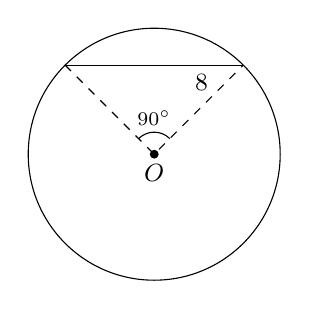
\begin{tikzpicture}[scale=0.8,font=\small]
\draw (0,0) circle (2); \fill (0,0) circle (2pt); \node[below] at (0,0) {$O$};
\coordinate (P) at (135:2); \coordinate (Q) at (45:2); \draw (P)--(Q); \draw[dashed] (P)--(0,0)--(Q);
\draw (0,0)++(45:0.35) arc (45:135:0.35); \node[above] at (0,0.3) {\scriptsize$90^\circ$}; \node[below] at (0.75,1.42) {$8$};
\end{tikzpicture}}
\Opts{$4$}{$2\sqrt2$}{$4\sqrt2$}{$8$}}
\QQ{24}{Quyidagi grafiklardan neçtasi funksiya böladi?
\qfig{\begin{tikzpicture}[scale=0.42,font=\small]
\foreach \dx/\dy/\n in {0/0/1,6.5/0/2,0/-6/3,6.5/-6/4} {\begin{scope}[shift={(\dx,\dy)}]
\draw[-{Stealth[length=3pt]}] (-2.5,0)--(2.5,0) node[below] {\scriptsize$x$}; \draw[-{Stealth[length=3pt]}] (0,-2.3)--(0,2.5) node[right] {\scriptsize$y$}; \node at (-2.4,2.2) {\n)};
\end{scope}}
\draw[thick] (0,0) circle (1.5); \draw[thick] (6.5+1.5,0) arc (0:180:1.5);
\draw[thick] (0,-6+1.5) arc (90:-90:1.5); \draw[thick,domain=-1.4:1.4,samples=40,shift={(6.5,-6)}] plot ({\x*\x-1.2},\x);
\end{tikzpicture}}
\Opts{$1$}{$2$}{$3$}{hammasi}}
\QQ{25}{$ABC$ töğri burçakli uçburçakning $B$ töğri burçak bissektrisasi $AC$ gipotenuzani $\sqrt5$ va $2\sqrt5$ kesmalarga ajratsa, $ABC$ töğri burçakli uçburçak yuzini toping.
\qfig{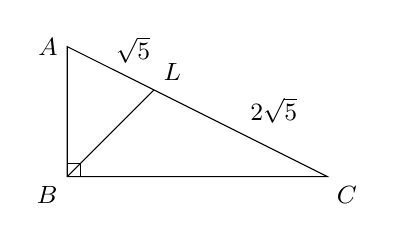
\begin{tikzpicture}[scale=0.55,font=\small]
\coordinate (B) at (0,0); \coordinate (A) at (0,3); \coordinate (C) at (6,0); \coordinate (L) at (2,2);
\draw (A)--(B)--(C)--cycle; \draw (B)--(L); \draw (0,0.3)--(0.3,0.3)--(0.3,0);
\node[left] at (A) {$A$}; \node[below left] at (B) {$B$}; \node[below right] at (C) {$C$}; \node[above right] at (L) {$L$};
\node[above right] at (0.9,2.4) {$\sqrt5$}; \node[above right] at (4,1) {$2\sqrt5$};
\end{tikzpicture}}
\Opts{$12$}{$9$}{$18$}{$15$}}
\QQ{26}{$ABC$ uçburçakning $A$ va $B$ uçlaridan $AD$ va $BE$ bissektrisalar tuşirildi. $BE$ va $AD$ bissektrisalar $K$ nuqtada kesişadi. Agar $AB=6$, $AE=4$ va $EC=8$ bölsa, $KDCE$ törtburçak yuzini toping.
\qfig{\begin{tikzpicture}[scale=0.5,font=\small]
\coordinate (A) at (0,0); \coordinate (C) at (12,0); \coordinate (B) at (1.5,5.809); \coordinate (E) at (4,0); \coordinate (D) at (5,3.873);
\coordinate (K) at (intersection of A--D and B--E);
\fill[qfill] (K)--(D)--(C)--(E)--cycle;
\draw (A)--(B)--(C)--cycle; \draw (A)--(D); \draw (B)--(E);
\node[below left] at (A) {$A$}; \node[above] at (B) {$B$}; \node[below right] at (C) {$C$}; \node[above right] at (D) {$D$}; \node[below] at (E) {$E$}; \node[above left] at (K) {$K$};
\node[left] at (0.75,2.9) {$6$}; \node[below] at (2,0) {$4$}; \node[below] at (8,0) {$8$};
\end{tikzpicture}}
\Opts{$\dfrac{26\sqrt{15}}5$}{$\dfrac{12\sqrt{15}}5$}{$\dfrac{24\sqrt{15}}5$}{$\dfrac{13\sqrt{15}}5$}}
\QQ{27}{$ABCD$ trapetsiyaning $BC$ va $AD$ asoslari mos ravişda $7$ va $27$ ga, $AB$ va $CD$ yon tomonlari esa mos ravişda $12$ va $16$ ga teng bölsa, $ABCD$ trapetsiya yuzini toping.
\qfig{\begin{tikzpicture}[scale=0.24,font=\small]
\coordinate (A) at (0,0); \coordinate (B) at (7.2,9.6); \coordinate (C) at (14.2,9.6); \coordinate (D) at (27,0);
\draw (A)--(B)--(C)--(D)--cycle;
\node[below left] at (A) {$A$}; \node[above left] at (B) {$B$}; \node[above right] at (C) {$C$}; \node[below right] at (D) {$D$};
\node[above] at (10.7,9.6) {$7$}; \node[below] at (13.5,0) {$27$}; \node[left] at (3.6,4.8) {$12$}; \node[right] at (20.6,4.8) {$16$};
\end{tikzpicture}}
\Opts{$163\dfrac15$}{$162\dfrac15$}{$161\dfrac15$}{$160\dfrac15$}}
\QQ{28}{Muntazam $n$ burçakning bir uçidan çiqqan eng kiçik diagonallari orasidagi burçak $120^\circ$ ga teng bölsa, muntazam $n$ burçakning neçta tomoni bor?
\qfig{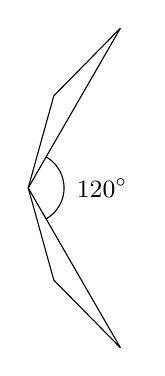
\begin{tikzpicture}[scale=1.3,font=\small]
\coordinate (V) at (0,0); \coordinate (P1) at (0.25,0.9); \coordinate (Q1) at (0.9,1.56); \coordinate (P2) at (0.25,-0.9); \coordinate (Q2) at (0.9,-1.56);
\draw (Q1)--(P1)--(V)--(P2)--(Q2); \draw (V)--(Q1); \draw (V)--(Q2);
\draw (V)++(60:0.35) arc (60:-60:0.35); \node[right] at (0.38,0) {$120^\circ$};
\end{tikzpicture}}
\Opts{$10$}{$12$}{$8$}{$16$}}
\QQ{29}{$ABC$ uçburçak dekart koordinatalar sistemasiga joylaştirildi. Uçburçak uçlarining koordinatalari $A(1;\,3)$, $B(5;\,1)$, $C(4;\,4)$ ga teng bölsa, $AL$ bissektrisa uzunligini toping.
\qfig{\begin{tikzpicture}[scale=0.7,font=\small]
\draw[-{Stealth[length=4pt]}] (-0.4,0)--(6,0) node[right] {$x$}; \draw[-{Stealth[length=4pt]}] (0,-0.4)--(0,4.8) node[left] {$y$};
\coordinate (A) at (1,3); \coordinate (B) at (5,1); \coordinate (C) at (4,4); \coordinate (L) at (4.414,2.757);
\draw (A)--(B)--(C)--cycle; \draw (A)--(L);
\node[left] at (A) {$A(1;3)$}; \node[below right] at (B) {$B(5;1)$}; \node[above] at (C) {$C(4;4)$}; \node[right] at (L) {$L$}; \node[below left] at (0,0) {$O$};
\end{tikzpicture}}
\Opts{$\sqrt{40-10\sqrt2}$}{$\sqrt{40-20\sqrt2}$}{$\sqrt{30-15\sqrt2}$}{$\sqrt{30-10\sqrt2}$}}
\QQ{30}{Muntazam törtburçakli piramidaning töla sirtining yuzi asosining yuzidan $3$ marta katta bölsa, yon yoği bilan asos tekisligi orasidagi burçak tangensini toping.
\Opts{$\dfrac12$}{$\dfrac1{\sqrt3}$}{$\sqrt3$}{$1$}}
\QQ{31}{$A=\{60\text{ ning natural böluvçilari}\}$, $B=\{48\text{ ning natural böluvçilari}\}$ bölsa, $A\cap B$ ning qism töplamlari sonini toping.
\Opts{$16$}{$32$}{$64$}{$128$}}
\QQ{32}{Raqamlar yiğindisi $7$ ga teng bölgan uç xonali sonlar qoğozçalarga yozilgan. Ulardan tanlangan son juft son böliş ehtimolligini toping.
\Opts{$\dfrac12$}{$\dfrac{15}{28}$}{$\dfrac34$}{$\dfrac47$}}
\QQ{33}{\Moslash{Rasmda konus içiga eng katta hajmli silindr içki çizilgan.
\par\centering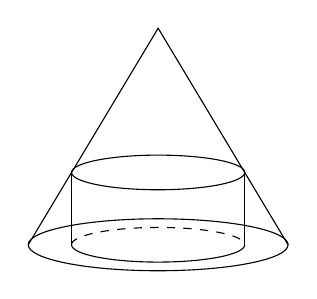
\begin{tikzpicture}[scale=0.55,font=\small]
\draw (0,0) ellipse (3 and 0.6); \draw (-3,0)--(0,5)--(3,0);
\draw (0,1.67) ellipse (2 and 0.4); \draw (-2,0)--(-2,1.67); \draw (2,0)--(2,1.67); \draw[dashed] (-2,0) arc (180:0:2 and 0.4); \draw (-2,0) arc (180:360:2 and 0.4);
\end{tikzpicture}}{A) $\dfrac13$\par B) $\dfrac23$\par C) $1$\par D) $\dfrac34$\par E) $\dfrac49$\par F) $\dfrac29$}{Silindr asosining radiusini konus asosi radiusiga nisbatini toping.}{Silindr balandligini konus balandligiga nisbatini toping.}{Silindr hajmini konus hajmiga nisbatini toping.}}
\QQ{36}{Tenglamalar sistemasini yeçing:
\[\begin{cases}26x^2+42xy+17y^2=10,\\ 10x^2+18xy+8y^2=6\end{cases}\]
\AB{Tenglamalar sistemasi yeçimlari $(x_1;y_1)$, $(x_2;y_2)$, \dots, $(x_n;y_n)$ bölsa, tenglamalar sistemasi neçta yeçimga ega?}{$x_n+y_n$ ning eng katta qiymatini toping.}}
\QQ{37}{Tenglamani yeçing:
\[\sin^3x+\sin^32x+\sin^33x=(\sin x+\sin2x+\sin3x)^3\]
\AB{Tenglamaning eng kiçik musbat ildizini toping.}{Tenglama $[-\pi;\,\pi]$ oraliqda neçta ildizga ega?}}
\QQ{38}{$f(x)=\dfrac{ax+b}{cx+d}$ funksiya $Ox$ öqini $(3;\,0)$ nuqtada kesib ötadi. Agar $f(x)$ funksiyaning qiymatlar sohasi $E(f)=(-\infty;\,2)\cup(2;\,\infty)$ va $f(x)=f^{-1}(x)$ bölsa ($f^{-1}(x)$ — $f(x)$ funksiyaning teskari funksiyasi),
\AB{$f(x)$ ning aniqlaniş sohasiga tegişli bölmagan sonni toping.}{$f^{-1}(6)$ ning qiymatini toping.}}
\QQ{39}{$f(x)=\dfrac{x^2}8-\dfrac{3x}2$ kvadrat funksiya va $x^2-18x+y^2-12y+97=0$ aylana tenglamasi berilgan.
\qfig{\begin{tikzpicture}[scale=0.3,font=\small]
\draw[-{Stealth[length=4pt]}] (-3,0)--(17,0) node[right] {$x$}; \draw[-{Stealth[length=4pt]}] (0,-5.5)--(0,11) node[left] {$y$};
\draw[thick,domain=-2.5:15,samples=60] plot (\x,{\x*\x/8-1.5*\x}); \draw[thick] (9,6) circle (4.472);
\fill (9,6) circle (5pt); \fill (6,-4.5) circle (5pt); \draw (9,6)--(6,-4.5); \node[left] at (7.3,0.8) {$d_1$};
\node[below left] at (0,0) {$O$}; \node[right] at (15,5.6) {$y=f(x)$};
\end{tikzpicture}}
\AB{Aylana markazi va parabola uçi orasidagi masofa $d_1$ ni toping.}{Paraboladan aylanagaça eng qisqa masofa $d_2$ ni toping.}}
\QQ{40}{$f(x)=-2x^2+4x$ va $g(x)=x^2+px+q$ funksiyalar grafiklari bilan çegaralangan soha yuzi $\dfrac{32}{27}$ ga teng. Agar $x=\dfrac43$ töğri çiziq çegaralangan sohani teng ikkiga ajratsa,
\AB{$f(x)$ va $g(x)$ funksiyalar kesişiş nuqtalari abssissalari yiğindisini toping.}{$p\cdot q$ ning qiymatini toping.}}
\QQ{41}{$ABC$ uçburçakka aylana içki çizilgan. $ABC$ uçburçakning $A$ uçidan $AD$ bissektrisa ötkazildi. $BC$ tomoniga parallel va aylana markazidan ötuvçi $EF$ kesma ötkazilgan ($E\in AB$, $F\in AC$). Agar $BC=30$, $EB=8$ va $FC=12$ bölsa,
\qfig{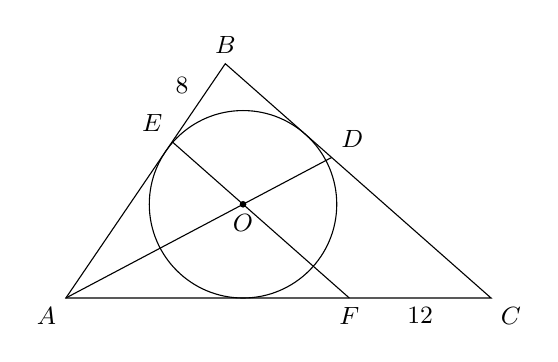
\begin{tikzpicture}[scale=0.15,font=\small]
\coordinate (A) at (0,0); \coordinate (C) at (36,0); \coordinate (B) at (13.5,19.84); \coordinate (O) at (15,7.936); \coordinate (E) at (9,13.23); \coordinate (F) at (24,0); \coordinate (D) at (22.5,11.9);
\draw (A)--(B)--(C)--cycle; \draw (O) circle (7.936); \draw (A)--(D); \draw (E)--(F); \fill (O) circle (8pt);
\node[below left] at (A) {$A$}; \node[above] at (B) {$B$}; \node[below right] at (C) {$C$}; \node[above right] at (D) {$D$}; \node[above left] at (E) {$E$}; \node[below] at (F) {$F$}; \node[below] at (O) {$O$};
\node[above left] at (11.2,16.5) {$8$}; \node[below] at (30,0) {$12$};
\end{tikzpicture}}
\AB{$DC$ kesma uzunligini toping.}{$AB$ va $AC$ tomonlari ayirmasi modulini toping.}}
\QQ{42}{$ABCD$ kvadrat içidan $P$ nuqta olingan. Agar $AP=1$, $BP=5$, $PC=7$ bölsa,
\qfig{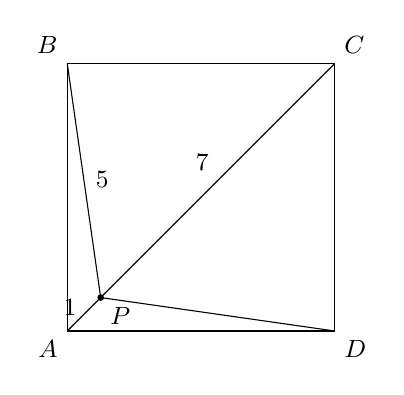
\begin{tikzpicture}[scale=0.6,font=\small]
\coordinate (A) at (0,0); \coordinate (B) at (0,5.657); \coordinate (C) at (5.657,5.657); \coordinate (D) at (5.657,0); \coordinate (P) at (0.707,0.707);
\draw (A)--(B)--(C)--(D)--cycle; \draw (A)--(P)--(B); \draw (P)--(C); \draw (P)--(D); \fill (P) circle (2pt);
\node[below left] at (A) {$A$}; \node[above left] at (B) {$B$}; \node[above right] at (C) {$C$}; \node[below right] at (D) {$D$}; \node[below right] at (P) {$P$};
\node[right] at (0.4,3.2) {$5$}; \node[above left] at (3.2,3.2) {$7$}; \node[left] at (0.4,0.5) {$1$};
\end{tikzpicture}}
\AB{$PD$ kesma uzunligini toping.}{Kvadratning yuzini toping.}}
\QQ{43}{Rasmda $ADFK$ parallelogramm va $EG:GC=1:2$, $DE:EF=2:3$ bölsin.
\qfig{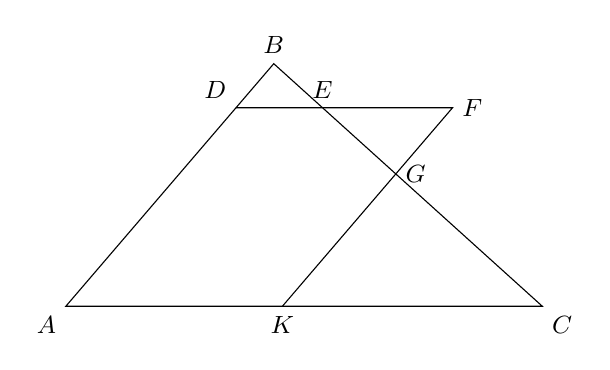
\begin{tikzpicture}[scale=0.55,font=\small]
\coordinate (A) at (0,0); \coordinate (B) at (4.8,5.6); \coordinate (C) at (11,0); \coordinate (D) at (3.927,4.582); \coordinate (E) at (5.927,4.582); \coordinate (F) at (8.927,4.582); \coordinate (K) at (5,0); \coordinate (G) at (7.618,3.055);
\draw (A)--(B)--(C)--cycle; \draw (D)--(F)--(K);
\node[below left] at (A) {$A$}; \node[above] at (B) {$B$}; \node[below right] at (C) {$C$}; \node[above left] at (D) {$D$}; \node[above] at (E) {$E$}; \node[right] at (F) {$F$}; \node[below] at (K) {$K$}; \node[right] at (G) {$G$};
\end{tikzpicture}}
\AB{$\dfrac{EG}{BC}$ ni toping.}{Agar $S_{ABC}=242$ bölsa, $S_{ADFK}$ ni toping.}}
\QQ{44}{$AB$ diametrli, radiusi $3$ ga teng bölgan sfera berilgan. $C$ va $D$ nuqtalar sferada joylaşgan. $DC$ qirrasi örtasidan $E$ nuqta olindi. Sferaga eng katta hajmli $ABCD$ piramida içki çizilgan bölsa,
\AB{Piramida hajmini toping.}{$AE$ çiziq va $ABC$ asos tekisligi orasidagi burçak sinusini toping.}}
\QQ{45}{Silindr şaklidagi yoğoç hajmi $V=162\pi$ cm$^3$ va yon sirti $S=72\pi$ cm$^2$ ga teng. Usta uni yönib şar şakliga keltirdi. Şarning hajmi eng katta bölsin ($\pi\approx3$ deb olinsin).
\qfig{\begin{tikzpicture}[scale=0.45,font=\small]
\draw (0,4.5) ellipse (3 and 0.6); \draw (-3,0)--(-3,4.5); \draw (3,0)--(3,4.5); \draw (-3,0) arc (180:360:3 and 0.6); \draw[dashed] (3,0) arc (0:180:3 and 0.6);
\fill[qfill] (0,2.25) circle (2.25); \draw (0,2.25) circle (2.25); \draw[dashed] (-2.25,2.25) arc (180:360:2.25 and 0.45);
\end{tikzpicture}}
\AB{Kesib olingan şar sirtining yuzini toping.}{Silindrdan eng katta şar kesib olinganda çiqindi hajmini toping.}}
\Javoblar{A C B A C B B C B B A C C A C D B C B C A B C A B C A B B C C D B A E}{\OK{36}{$4$}{$3$}\OK{37}{$\dfrac{2\pi}5$}{$11$}\OK{38}{$2$}{$\dfrac32$}\OK{39}{$\dfrac{3\sqrt{53}}2$}{$\dfrac{\sqrt5}2$}\OK{40}{$\dfrac83$}{$-16$}\OK{41}{$18$}{$12$}\OK{42}{$5$}{$32$}\OK{43}{$\dfrac3{11}$}{$180$}\OK{44}{$9$}{$\dfrac{\sqrt6}6$}\OK{45}{$192$ cm$^2$}{$230$ cm$^3$}}
